\ifx\bookloaded\undefined
\documentclass{article}
\usepackage{graphicx}
\usepackage{tikz}
\usetikzlibrary{snakes}
\usetikzlibrary{arrows}
\usetikzlibrary{shapes}
\usetikzlibrary{backgrounds}
\input book_defs
\begin{document}
\fi
\section{Chapter 3}
\begin{enumerate}
\item{\bf Constant Velocity Charge}

Show that if charge is not accelerating, the electric field vector
points to the current (not the retarded) position of the charge.

{\bf Answer:}

\begin{center}
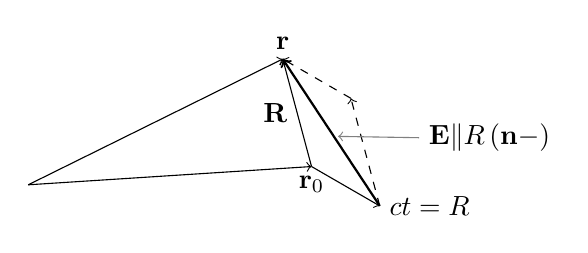
\begin{tikzpicture}
\begin{scope}[rotate=-30]
\draw [->] (0,0)--(2,3);
\draw [->] (0,0)--(3,2);
\draw [->] (3,2)--(4,2) ;
\draw [->] (3,2)--(2,3) ;
\draw [->,dashed] (4,2)--(3,3) ;
\draw [->,dashed] (3,3)--(2,3) ;
\draw [->,thick] (4,2)--(2,3) ; 
\draw (3,2) node [below] {${\bf r}_0$} 
(4,2) node [right] {$\betabold c t=\betabold R$} 
(2,3) node [above] {${\bf r}$} 
(2.5,2.5) node [left] {${\bf R}$}
(4,3) node [right] {${\bf E} \| R\left ({\bf n}-\betabold\right)$};
\draw [->,gray] (4,3)--(3.1,2.5);
\end{scope}
\end{tikzpicture}
\end{center}

\setcounter{enumi}{3}

\item{\bf Synchrotron Cooling:}

A particle of mass $m$, charge $q$, moves in a plane perpendicular to
a uniform, static, magnetic field $B$.
\begin{enumerate}
\item
Calculate the total energy radiated per unit time, expressing it in
terms of the constants already defined and the ratio
$\gamma=1/\sqrt{1-\beta^2}$ of the particle's total energy to its rest 
energy.  You can assume that the particle is ultrarelativistic.
\item
If at time $t=0$ the particle has a total energy $E_0=\gamma_0 m c^2$,
show that it will have energy $E=\gamma m c^2 < E_0$ at a time $t$,
where
\[
t \approx \frac{3 m^3 c^5}{2 q^4 B^2} \left ( \frac{1}{\gamma} -
\frac{1}{\gamma_0} \right ).
\]
\end{enumerate}

{\bf Answer:}

The synchrotron power is given by the power emitted by a particle
performing circular motion
$$
P_\perp = \frac{2}{3} \frac{q^2}{m^2 c^3} \gamma^2 \left ( \frac{d
    {\bf p}}{dt} \right )^2
$$
where for an ultrarelativistic charged particle in a magnetic field we
have
$$
\left | \frac{d {\bf p}}{dt} \right | = q B
$$
so
$$
P_\perp =  \frac{2}{3} \frac{q^5}{m^2 c^3} \gamma^2 B^2 = -\frac{d
  E}{dt} = -m c^2 \frac{d \gamma}{dt}
$$
and
$$
\frac{d \gamma}{dt} = -\frac{2}{3} \frac{q^5}{m^3 c^5} B^2 \gamma^2.
$$
Separating the variables and integrating yields the required answer.

\item{\bf Classical HI:}
A particle of mass $m$ and charge $q$ moves in a circle due to a force 
${\bf F} = -\hat{\bf r} \frac{q^2}{r^2}$.  
You may assume that the particle always moves  non-relativistically.
\begin{enumerate}
\item What is the acceleration of the particle as a function of $r$?
\item What is the total energy of the particle as a function of $r$?
  The potential energy is given by $-q^2/r$.
\item What is the power radiated as a function of $r$?
\item Using the fact the $P=-dE/dt$ and the answer to (2), find
  $dr/dt$. 
\item Assuming that the particle starts with $r=r_i$ at $t=0$, find
  the value of $t$ where $r=0$.   
\item Let's assume that $q=e$, the charge of the electron, and
  $m=m_e$, the mass of the electron.  Write your answer in (4) in
  terms of $r_i$, $r_0$ (the classical electron radius) and $c$.
\item What is the time if $r_i=0.5$\AA (for an hydrogen)?
\item Compare this to the lifetime of a hydrogen atom.
\end{enumerate}

{\bf Answer:}

\begin{enumerate}
\item 
\[ \dot{\bf u} = -{\hat r} \frac{q^2}{r^2 m} \]
\item
\[ E = -\frac{q^2}{r} + \frac{1}{2} m v^2 = -\frac{q^2}{r} + \frac{1}{2} \left ( \frac{q^2}{r} \right ) = -\frac{1}{2} \frac{q^2}{r} \]
where I used
\[ \frac{m v^2}{r} = \frac{q^2}{r^2} \]
for circular motion.
\item 
\[
P = \frac{2 q^2 \dot{u}^2}{3 c^3} = \frac{2 q^2 }{3 c^3} \left ( \frac{q^2}{r^2 m} \right )^2
\]
\item 
\[ 
\frac{d E}{d t} = \frac{d}{dt} \left ( -\frac{1}{2} \frac{q^2}{r} \right ) = \frac{1}{2} \frac{q^2}{r^2} \frac{dr}{dt}
\]
\[
\frac{d E}{d t} = -P =  -\frac{2 q^6 }{3 m^2 c^3} \frac{1}{r^4} =  \frac{1}{2} \frac{q^2}{r^2} \frac{dr}{dt}
\]
\[
 \frac{dr}{dt} =  -\frac{4 q^4 }{3 m^2 c^3} \frac{1}{r^2}
\]
\item
\[
t = \int_{r_i}^0 \frac{dt}{dr} dr = -\frac{3 m^2 c^3}{4 q^4 }\int_{r_i}^0 r^2 d r
=  \frac{ r_i^3 m^2 c^3}{4 q^4 }
\]
\item
\[
t =  \frac{ r_i^3 m^2 c^3}{4 e^4 } = \frac{1}{4 c} r_i \left ( \frac{r_i}{r_0} \right )^2
\]
\item
\[
r_0 = 2.82 \times 10^{-13}~\rmmat{cm}, 1\rmmat{\AA} = 10^{-8}~\rmmat{cm}
\]
\[
t = \frac{1}{12 \times 10^{10} \rmmat{cm/s}} 0.5 \times 10^{-8}~\rmmat{cm}  ( 17000 )^2 = 1.2 \times 10^{-11}~\rmmat{s}
\]
\item
It is much smaller than the lifetime of a hydrogen atom.
\end{enumerate}

\item{\bf The Eddington Luminosity:} 

  There is a natural limit to the luminosity a gravitationally bound
  object can emit. At this limit the inward gravitational force on a
  piece of material is balanced by the outgoing radiation
  pressure. Although this limiting luminosity, the Eddington
  luminosity, can be evaded in various ways, it can provide a useful
  (if not truly firm) estimate of the minimum mass of a particular
  source of radiation.

\begin{enumerate}
\item Consider ionized hydrogen gas. Each electron-proton pair has a
  mass more or less equal to the mass of the proton ($m_p$) and a cross
  section to radiation equal to the Thompson cross-section ($\sigma_T$).
\item The radiation pressure is given by outgoing radiation flux over the speed of light.
\item Equate the outgoing force due to radiation on the pair with the inward force of gravity on the pair.
\item Solve for the luminosity as a function of mass.
\end{enumerate}
The mass of the sun is $2 \times 10^{33}$g. What is the Eddington
luminosity of the sun?

{\bf Answer:}
\begin{enumerate}
\item OK
\item $P=\frac{F}{c} = \frac{L}{4\pi r^2 c}$
\item $F_\mathrm{out} = P \sigma_T = \frac{L \sigma_T}{4\pi r^2 c}$,
  $F_\mathrm{in} = \frac{G M m_p}{r^2}$
\item
  $F_\mathrm{in}=F_\mathrm{out}$ for $L=L_\mathrm{Edd}$ so
  $L_\mathrm{Edd} = \frac{4\pi c G M m_p}{\sigma_T}$
\item
  $L_\mathrm{Edd} = 1.26 \times 10^{38} \textrm{erg/s} \left (\frac{M}{M_\odot}
  \right ) = 3.2 \times 10^4 \left (\frac{M}{M_\odot}
  \right ) L_\odot.$
\end{enumerate}
\end{enumerate}


\ifx\bookloaded\undefined
\end{document}
\end
\fi
%%% Local Variables:
%%% TeX-master: "book"
%%% End: